%%%%%%%%%%%%%%%%%%%%%%%%%%%%%%%%%%%%%%%%%%%%%%%%%%%%%%%%%%%%%%%%%%%%%
% LaTeX Template: Project Modified (v 0.2) by jluo
%
% Original Source: http://www.howtotex.com
% Date: February 2019
% 
% This is a title page template which be used for articles & reports.
% 
% 
%%%%%%%%%%%%%%%%%%%%%%%%%%%%%%%%%%%%%%%%%%%%%%%%%%%%%%%%%%%%%%%%%%%%%%

\documentclass[12pt]{report}
\usepackage[a4paper]{geometry}
\usepackage[myheadings]{fullpage}
\usepackage{fancyhdr}
\usepackage{lastpage}
\usepackage{graphicx, wrapfig, subcaption, setspace, booktabs}
\usepackage{fourier}
\usepackage[protrusion=true, expansion=true]{microtype}
\usepackage[english]{babel}
\usepackage{sectsty}
\usepackage{url, lipsum}
\usepackage{tgbonum}
\usepackage{hyperref}
\usepackage[table]{xcolor}
\usepackage{listings}
\usepackage{color}
\usepackage[default]{lato}
\usepackage[T1]{fontenc}
\usepackage{titlesec}
\usepackage{multirow}

\definecolor{codegreen}{rgb}{0,0.6,0}
\definecolor{codegray}{rgb}{0.5,0.5,0.5}
\definecolor{codepurple}{rgb}{0.58,0,0.82}
\definecolor{backcolour}{rgb}{0.95,0.95,0.92}
\definecolor{dkgreen}{rgb}{0,.6,0}
\definecolor{dkblue}{rgb}{0,0,.6}
\definecolor{dkyellow}{cmyk}{0,0,.8,.3}
\definecolor{mygray}{rgb}{0.5,0.5,0.5}


\lstset {
	breaklines=true,
	upquote=true
}

\lstdefinestyle{PHP}{
	language = php,
	backgroundcolor=\color{backcolour},
	basicstyle = \small\ttfamily,
	numbers=left,                    
	numbersep=5pt,
	numberstyle=\tiny\color{mygray},
	tabsize = 2,
	upquote=true,
	keywordstyle = \color{dkblue},
	stringstyle = \color{red},
	identifierstyle = \color{dkgreen},
	commentstyle = \color{gray},
	emph = [1]{php},
	emphstyle = [1]\color{black},
	emph = [2]{if,and,or,else},
	emphstyle = [2]\color{dkyellow},
	showspaces=false,
	showstringspaces=false
}

\onehalfspacing
\setcounter{tocdepth}{5}
\setcounter{secnumdepth}{5}

% set chapter format
\titleformat{\chapter}[block]
{\normalfont\huge\lato}{\thechapter}{1em}{\Huge}
\titlespacing*{\chapter}{0pt}{-19pt}{0pt}

% remove red boxes
\hypersetup{%
	pdfborder = {0 0 0}
}

% change the link style you can use 
\newcommand{\link}[1]{{\color{blue}\href{#1}{#1}}}

%-------------------------------------------------------------------------------
% HEADER & FOOTER
%-------------------------------------------------------------------------------
\pagestyle{fancy}
\setlength\headheight{15pt}
\fancyhead[L]{Company X Penetration Test}
\fancyhead[R]{Name Surname}

%-------------------------------------------------------------------------------
% TITLE PAGE
%-------------------------------------------------------------------------------
\title{Company X Penetration Test}
\author{Name Surname}

\makeatletter
\renewcommand{\maketitle}{
	\begin{titlepage}
		\begin{center}
			
\includegraphics[width=0.6\textwidth]{img/logo.png}\\
			\large
			\vspace*{1cm}
			{\LARGE\@title}
			\par\vspace{1ex}
			\begin{tabular}[t]{c}
				by \@author
			\end{tabular}
			\vfill
			\par\vspace{1ex}
			Start of testing: February 13, 2019\\
			End of testing: February 20, 2019\\
		\end{center}
		\@thanks
	\end{titlepage}
}
\makeatother

\begin{document}
		\maketitle
		
		% nessuna numerazione
		\pagenumbering{gobble} 
		\tableofcontents
		\newpage
		
		%-------------------------------------------------------------------------------
		% BODY
		%-------------------------------------------------------------------------------
		\pagenumbering{arabic} 
		\chapter{Executive Summary}

In this penetration test, the provided VM by the lecturer was assessed for security vulnerabilities. 
The assessment was conducted between the 18th February and the 18th March as a black box test, 
thus, no specific information about the internals of the system were provided. The scope of the assessment was as follows:
\begin{itemize}
	\item Virtual Machine: 10.1.0.10
\end{itemize}
As a result, several vulnerabilities have been identified among the assets of the VM, some of which pose a significant risk.
We found a few services running on the machine, which makes it vulnerable to exterior threats.
Two of these vulnerabilities \ref{weak_password} and \ref{management_server} are highly critical and allow an adversary to gain full access to the VM with all permissions, 
which would have a severe impact on the system. 
The solutions to these two vulnerabilities are not complicated and should be the top priority.

Other threats can be mitigated easily by keeping the system up to date and taking services offline that are not in use.
Therefore, we recommend reviewing the services you need to run on this machine.
Unnecessary services should be turned off, and the ones kept should be updated to the newest version. 

Solutions to remedy the discovered vulnerabilities are provided together with detailed descriptions and reproduction steps in chapter 3.

\begin{figure}[h]
	\centering
	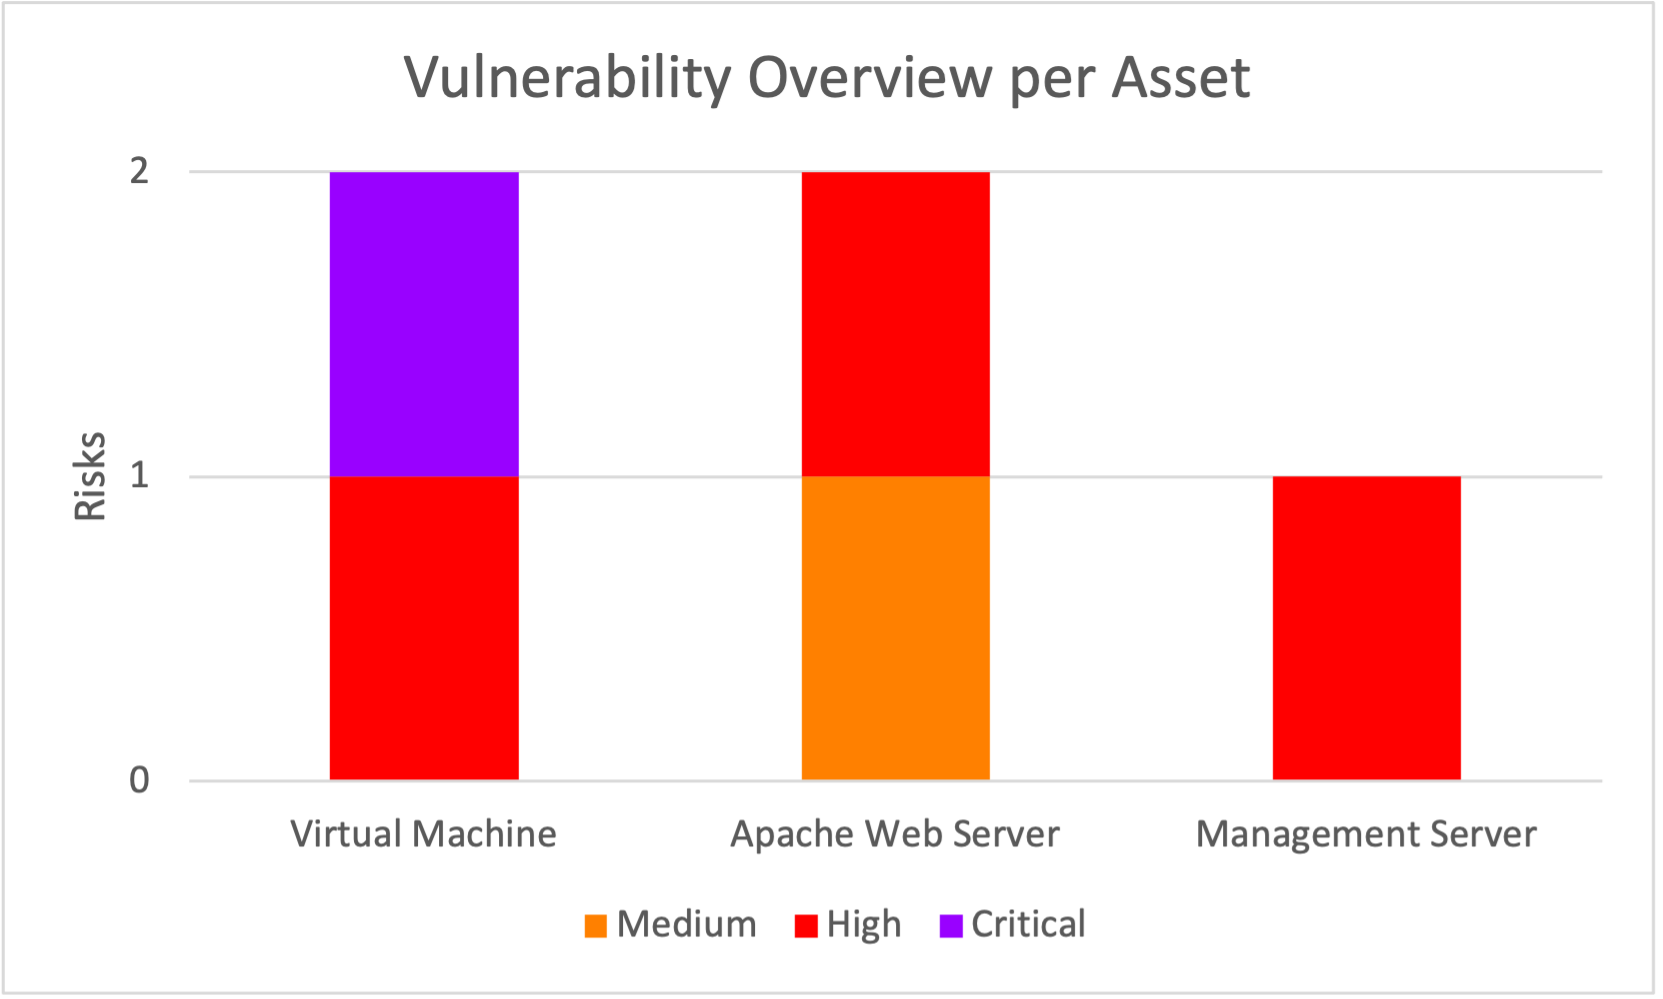
\includegraphics[width=13.5cm]{img/vuln_chart.png}
	\caption{Vulnerability Overview}
\end{figure}
	
		\newpage
		
		\chapter{Vulnerability overview}
Table \ref{tbl:vuln overview} depicts all vulnerabilities found during the penetration test. They are categorized by their risk and potential and are differentiated in the categories low, medium, high and critical. 

Here describe what severities are and what do they mean in context of your report. It's better to keep the color code across all the report.

Figure  shows the overview of vulnerabilities grouped by target.

\begin{figure}[h]
\centering
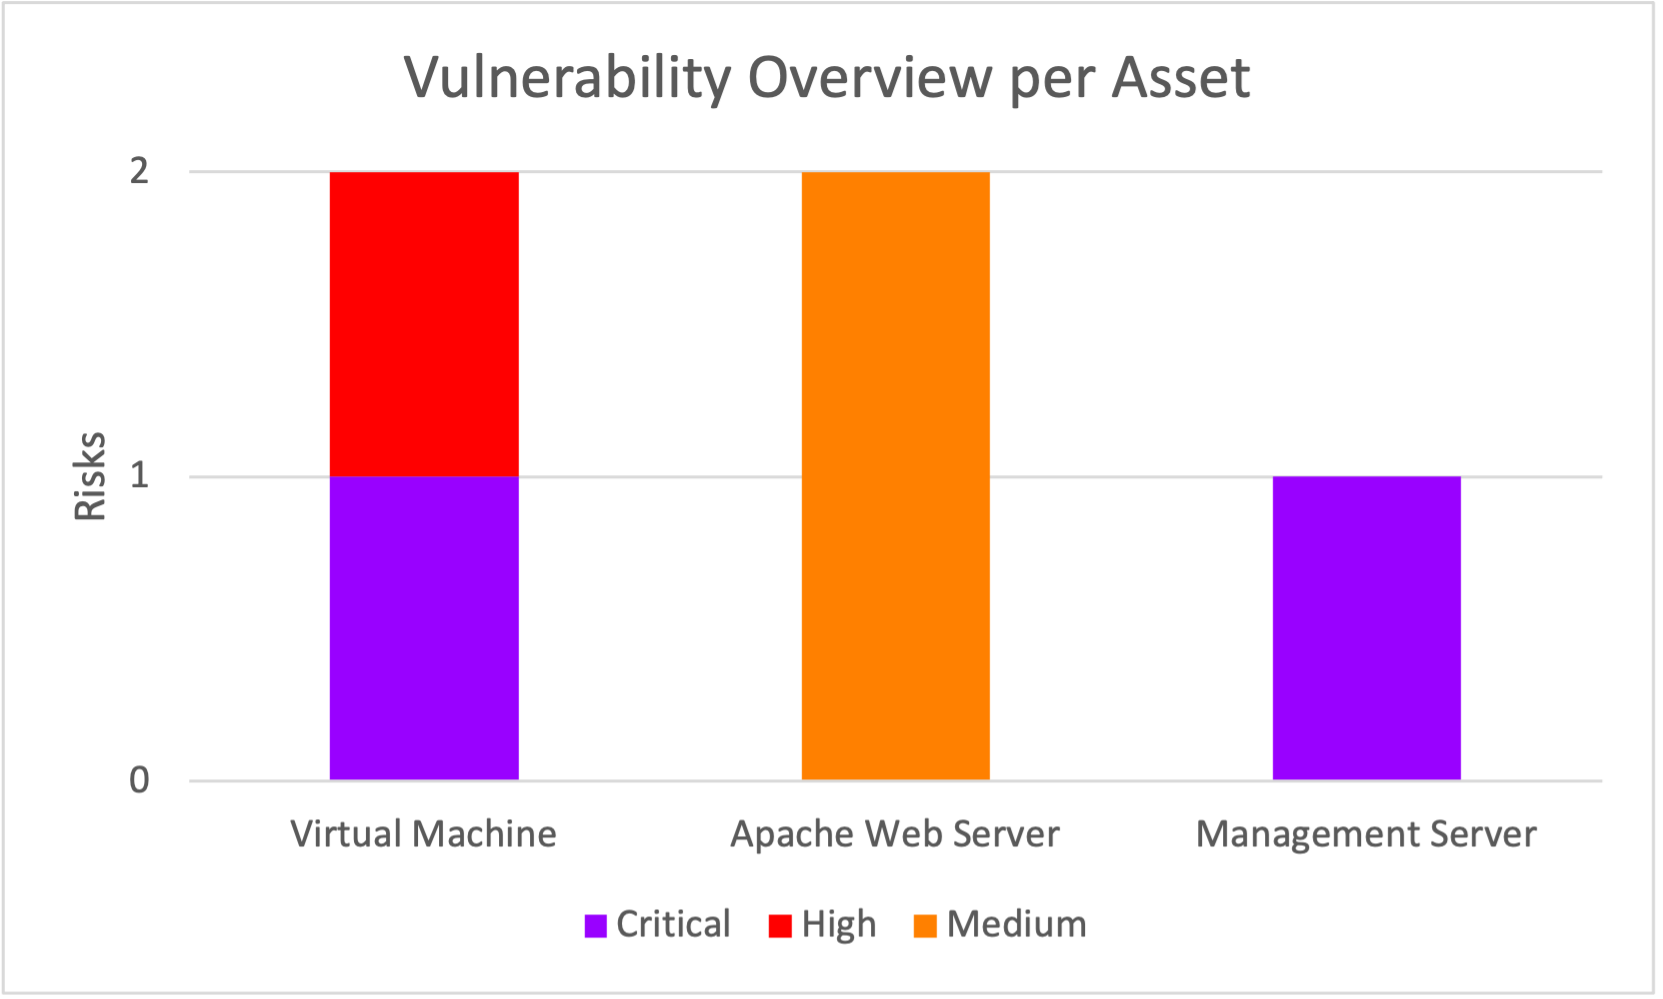
\includegraphics[width=\textwidth]{img/vulnerability_chart.png}
\caption{Vulnerability Overview}
\end{figure}

\begin{table}[h]
	\begin{tabular}{| l | l | p{7cm} | l | l |}
		\hline 
		Risk & Asset & Vulnerability & Section & Page\\
		\hline 
		\cellcolor{codepurple}Critical & Virtual Machine & Weak Password &  \ref{weak_password} & \pageref{weak_password} \\
		\hline 
		\cellcolor{red}High & Virtual Machine & Privilege Escalation &  \ref{privilege_escalation}& \pageref{privilege_escalation}\\
		\hline 
		\cellcolor{orange}Medium & Apache Web Server & Outdated Version &  \ref{outdated_version} & \pageref{outdated_version} \\
		\hline 
		\cellcolor{orange}Medium & Apache Web Server & Information Disclosure & \ref{information_disclosure} & \pageref{information_disclosure} \\
		\hline
		\cellcolor{codepurple}Critical & Management Server & Broken Authentication & \ref{management_server} & \pageref{management_server}\\
		\hline 
	\end{tabular}
	\caption{Vulnerability Overview}
	\label{tbl:vuln overview}
\end{table}
		\newpage
		
		\chapter{Results}
In this chapter, the vulnerabilities found during the penetration test are presented in detail. All issues are grouped by their target and contain the following information:
\begin{itemize}
	\item Brief description.
	\item CVSS Base Score -- see \href{https://www.first.org/cvss/user-guide}{\textcolor{blue}{\underline{here}}} for details.
	\item Exploitability -- describes the likelihood of an issue being used against customer's infrastructure.
	\item References to classifications: WASC, OWASP, CWE.
	\item Steps to reproduce.
\end{itemize}

Furthermore, recommendations for remediation are given for each vulnerability found during the penetration test. 
Both "quick win" and long-term solutions are presented as well as some code examples.

\section{Virtual Machine}
\textbf{Server IPv4 address}: 10.1.0.10\\
\textbf{Server IPv6 address}: fd01::a

\subsection{Open Ports}\label{open_ports}
The first step of our penetration test was scanning for open ports on the given virtual machine to get a starting point for 
our investigation. The port scanning was done with \textbf{nmap} on all ports of the VM. The scan had the following results:

\begin{minipage}{\linewidth}
\begin{verbatim}
	$ nmap -A -p 0-65535 10.1.0.10

	Nmap scan report for 10.1.0.10
	Host is up (0.018s latency).
	Not shown: 65533 closed tcp ports (conn-refused)
	PORT      STATE SERVICE VERSION
	22/tcp    open  ssh     OpenSSH 8.4p1 Debian 5 (protocol 2.0)
	| ssh-hostkey: 
	|   3072 e9:b7:ab:3a:b8:68:5e:cc:85:f6:00:b3:99:b9:22:ae (RSA)
	|   256 b4:7c:1f:96:22:5a:63:4d:2b:30:db:5f:ef:70:11:bd (ECDSA)
	|_  256 9d:40:34:55:05:70:80:b0:d0:ce:d0:d5:f4:5d:cd:28 (ED25519)
	80/tcp    open  http    Apache httpd 2.4.51 ((Debian))
	|_http-title: Apache2 Debian Default Page: It works
	|_http-server-header: Apache/2.4.51 (Debian)
	20321/tcp open  unknown
	Service Info: OS: Linux; CPE: cpe:/o:linux:linux_kernel
\end{verbatim}
\end{minipage}
\\
\\
With this scan we learned the operating system and revealed the open ports of the VM.
The port 22 is open and running the SSH-Service on version OpenSSH 8.4p1 Debian 5.
The VM also runs an \hyperref[apache]{\textcolor{blue}{\underline{Apache2-Server}}} with the version httpd 2.4.51 on port 80.
There is also running an unknown service on \hyperref[management_server]{\textcolor{blue}{\underline{open port 20321}}}.
These open ports will be the starting point of our penetration test.   

\subsection{Weak Password} \label{weak_password}
\begin{table}[h]
	\centering
	\begin{tabular}{| l | p{10cm} |}
		\hline 
		Description & The user bluey uses a weak password which can be brute-forced using common wordlists. \\
		\hline 
		CVSS Base Score & 9.1 \\
		\hline 
		Exploitablity & High \\
		\hline 
		References to classifications & A2:2017-Broken Authentication \\
		\hline 
	\end{tabular}
	\caption{Issue \#1: Weak password on Virtual Machine}
	\label{tbl:issue-1}
\end{table}

\subsubsection{Minimal proof of concept}
A curated list of users can be found on the Apache web server \ref{ss: issue-4}.
This led us to beliefe that those are the usernames of the given virtual machine.
We try to log in using the usernames and the rockyou wordlist on the open SSH port.
The tool used for the brute-force operation is hydra. We tried all usernames but only one was successful, due to the fact that \textit{root} is not accessible through SSH and \textit{bingo} is not an initialized user.    

\begin{verbatim}
$ hydra -l bluey -P rockyou.txt -t 4 10.1.0.10 ssh
\end{verbatim}

\subsubsection{Proposed solutions}
Use passwordless SSH authentication and disable password authentication

\subsection{Privilege Escalation} \label{privilege_escalation}
\begin{table}[h]
	\centering
	\begin{tabular}{| l | p{10cm} |}
		\hline 
		Description & The user bluey is able to read a log file using \colorbox{gray}{\lstinline[basicstyle=\ttfamily\color{white}]|less|} with root privilege. \\
		\hline 
		CVSS Base Score & 7.3 \\
		\hline 
		Exploitablity & High \\
		\hline 
		References to classifications & A01:2021 - Broken Access Control\\
		\hline 
	\end{tabular}
	\caption{Issue \#2}
\end{table}

\subsubsection{Minimal proof of concept}
Using the gained user account in \ref{ss: issue-1} we can investigate the virtual machine further. Since the user has no root privileges, we look for an application we can run as root without a password. In \colorbox{gray}{\lstinline[basicstyle=\ttfamily\color{white}]|etc/sudoers|} file we find the following line:
\begin{verbatim}
	bluey ALL=NOPASSWD: /usr/bin/less /var/log/auth.log
\end{verbatim}
This reveals the user bluey has root privileges to use \colorbox{gray}{\lstinline[basicstyle=\ttfamily\color{white}]|less|} on the \colorbox{gray}{\lstinline[basicstyle=\ttfamily\color{white}]|/var/log/auth.log|} file. This poses a huge vulnerability because \colorbox{gray}{\lstinline[basicstyle=\ttfamily\color{white}]|less|} allows a user to run commands inside the programm.
If we execute:
\begin{verbatim}
	!/bin/sh
\end{verbatim}
we start a new shell instance with root privileges since less was run with root privileges.
This means we now have full access on the virtual machine.

\subsubsection{Proposed solutions}


\section{Apache Web Server}\label{apache}
\textbf{Hostname \& Port}: 10.1.0.10:80\\
\\
With the \hyperref[open_ports]{\textcolor{blue}{\underline{initial port scanning}}}, we found a running Apache web server on port 80.
By using \textbf{nmap} we were able to retrieve the version of the web server which is used.
The Apache2 version on the VM is v.2.4.51 which was released in October 2021.
The web server is apparently not configured. When opening the web page in a browser, the Apache2 default index page is loaded.
\subsection{Outdated Version}
\begin{table}[h]
	\centering
	\begin{tabular}{| l | p{10cm} |}
		\hline 
		Description & Web server is vulnerable and outdated \\
		\hline 
		CVSS Base Score & 7.5 \\
		\hline 
		Exploitablity & Medium \\
		\hline 
		References to classifications & OWASP: A06:2021-Vulnerable and Outdated Components \\
		\hline
	\end{tabular}
	\caption{Issue \#3}
\end{table}

\subsubsection{Minimal proof of concept}
The Apache2 web server is featuring the version 2.4.51. There are several vulnerabilities for this version known by the Apache Software Foundation.
These vulnerabilities were only fixed in the more recent versions 2.4.52 and 2.4.53. You can find a detailed list of the vulnerabilities
\href{https://httpd.apache.org/security/vulnerabilities_24.html}{\textcolor{blue}{\underline{here}}}. \\
The following CVE entries apply to this version of Apache2:

\begin{itemize}
	\item \href{https://cve.mitre.org/cgi-bin/cvename.cgi?name=CVE-2021-44224}{\textcolor{blue}{\underline{CVE-2021-44224}}}:
	Possible NULL dereference or SSRF in forward proxy configurations in Apache HTTP Server 2.4.51 and earlier (moderate)

	\item \href{https://cve.mitre.org/cgi-bin/cvename.cgi?name=CVE-2021-44790}{\textcolor{blue}{\underline{CVE-2021-44790}}}
	Possible buffer overflow when parsing multipart content in mod\_lua of Apache HTTP Server 2.4.51 and earlier (important)

	\item \href{https://cve.mitre.org/cgi-bin/cvename.cgi?name=CVE-2021-22719}{\textcolor{blue}{\underline{CVE-2021-22719}}}:
	mod\_lua Use of uninitialized value of in r:parsebody (moderate)

	\item \href{https://cve.mitre.org/cgi-bin/cvename.cgi?name=CVE-2021-22720}{\textcolor{blue}{\underline{CVE-2021-22720}}}:
	HTTP request smuggling vulnerability in Apache HTTP Server 2.4.52 and earlier (important)

	\item \href{https://cve.mitre.org/cgi-bin/cvename.cgi?name=CVE-2021-22721}{\textcolor{blue}{\underline{CVE-2021-22721}}}:
	core: Possible buffer overflow with very large or unlimited LimitXMLRequestBody (low)

	\item \href{https://cve.mitre.org/cgi-bin/cvename.cgi?name=CVE-2021-23943}{\textcolor{blue}{\underline{CVE-2021-23943}}}:
	mod\_sed: Read/write beyond bounds (important)
\end{itemize}

\subsubsection{Proposed solutions}
We recommend upgrading the Apache2 web server to the newest version (currently v.2.4.53) where the vulnerabilities mentioned above have been fixed.
Since the web server is not configured and in use, it would be better to turn it off completely. It is just an unnecessary attack vector.
This would also mitigate the information disclosure in the following finding.

\subsection{Information Disclosure}\label{information_disclosure}
\begin{table}[h]
	\centering
	\begin{tabular}{| l | p{10cm} |}
		\hline 
		Description & Web server exposes usernames \\
		\hline 
		CVSS Base Score & 6.5 \\
		\hline 
		Exploitablity & Medium \\
		\hline 
		References to classifications & OWASP: A3:2017-Sensitive Data Exposure \\
		\hline
	\end{tabular}
	\caption{Issue \#4}
\end{table}

\subsubsection{Minimal proof of concept}
To find all subdomains of the web server we ran gobuster:

\begin{verbatim}
$ gobuster dir -u 10.1.0.10:80 -w /wordlists/dirbig.txt
\end{verbatim}
\vdots
\begin{verbatim}
===============================================================
//                    (Status: 200) [Size: 10701]
/home                 (Status: 301) [Size: 305] [--> http://10.1.0.10/home/]

===============================================================
\end{verbatim}
\vdots

Opening \url{10.1.0.10:80/home} in the browser reveals three potential usernames:
\begin{itemize}
	\item root
	\item bluey
	\item bingo
\end{itemize}

Each user is the label of a directory and we ran another subdomain enumeration per user:

\begin{verbatim}
	$ gobuster dir -u 10.1.0.10/home -w wordlists/file+dir.txt
\end{verbatim}
\vdots
\begin{verbatim}
	===============================================================
/root                 (Status: 301) [Size: 310] [--> http://10.1.0.10/home/root/]
/.htpasswd            (Status: 403) [Size: 274]
/.htaccess            (Status: 403) [Size: 274]
/.htpasswds           (Status: 403) [Size: 274]

===============================================================
\end{verbatim}
\vdots

as seen in the output the files that return are forbidden.

\subsubsection{Proposed solutions}
Proposed solution to the issue goes here.

\section{Management Server}\label{management_server}
\textbf{Hostname \& Port}: 10.1.0.10:20321\\
\\
The \hyperref[open_ports]{\textcolor{blue}{\underline{initial port scanning}}} revealed an unknown service on port 20321.
After breaking the password of the user "bluey" and logging into the virtual machine, we can look at the running processes.
There are two processes particularly interesting regarding the open port 20321:
\begin{verbatim}
	$ ps aux

	root      233604  0.0  0.4  17044  9560 ?        Ss   14:13   0:00 
	/usr/bin/python3 /opt/mgmtserver/mgmtserver \
		   { "certfile": "/etc/management-server/server.crt", \
		     "keyfile": "/etc/management-server/server.key" }
	
	root      233605  0.0  0.2   6928  4244 ?        S    14:13   0:00 
	/usr/bin/openssl s_server -accept 20321  \
		   -cert /etc/management-server/server.crt \
		   -key /etc/management-server/server.key -naccept 1 -Verify 1
\end{verbatim}
We can see that an SSL/TLS-Server from OpenSSL is running on port 20321.
From the results above and the certificate and key path, we can deduce that the two processes are connected.
It is highly probable that the SSL/TLS-Server is spawned by the python script "mgmtserver".
With the user "bluey" we can not access the mgmtserver directory.
To open the mgmtserver file, you need root access. For this, we can use the root user obtained with the 
\hyperref[privilege_escalation]{\textcolor{blue}{\underline{less exploit}}}.
In the code, we can see that the certificate is not validated with a root certificate. 
The subject of the client certificate is only compared with another string.
\\
\\
\begin{minipage}{\linewidth}
	\begin{verbatim}
		...
		if self._client_cert == "subject=CN = Management Client Certificate, \
			O = Secure Systems Inc., OU = admin=false":
		...
		elif self._client_cert == "subject=CN = Management Client Certificate, \
			O = Secure Systems Inc., OU = admin=true":
		...
	\end{verbatim}
\end{minipage}
\\
\subsubsection{Minimal proof of concept}
We can easily create a self-signed certificate that satisfies this string comparison. Such a certificate can be created with the following
OpenSSL command:
\begin{verbatim}
$ openssl req -newkey rsa:4096 \                                              
	  -x509 \
	  -sha256 \
	  -subj "/CN=Management Client Certificate/O=Secure Systems Inc./OU=admin=true" \ 
	  -days 3650 \
	  -nodes \
	  -out example.crt \
	  -keyout example.key
\end{verbatim}
With the certificate which can be created with the above command, we can now connect to port 20321. The python script will now compare the subject
of our client certificate with the string in the file and grant root access to the VM. To connect to the port, we can use the OpenSSL-Client:
\begin{verbatim}
	$ openssl s_client -connect 10.1.0.10:20321 -cert example.crt -key example.key
\end{verbatim}
\subsubsection{Proposed solutions}
To solve this vulnerability and improve the authentication, we recommend to not make a simple string comparison with the client certificate subject
and instead verify the client certificate with a root certificate you own. You can create a self-signed certificate and use it as a certificate 
authority. This CA certificate will be used to issue client certificates with which you can connect to your management server.
For authentication, you just have to verify the digital signature on the client certificate if it was issued by your root certificate. 

\newpage
		\newpage
		
		\chapter{Appendices} 

\section{Appendix \#1} \label{appendix-1}
Appendix 1.

\section{Appendix \#2} \label{appendix-2}
Appendix 2.
\end{document}